\chapter{Balancing Map Compression with Information Accuracy}
\label{chapter4}

This chapter examines distortions to mutual information between a sensor
measurement and a map when the map undergoes compression. The PRI
compression strategy described in Chapter~\ref{chapter3} is lossy, resulting in
compressed maps that have a lower information content than their uncompressed
originators. It should be expected, then, that information about
random variables that share a dependence with the map (such as a sensor measurement) is also lost
when the map undergoes compression. Large distortions to a mutual information reward metric
(e.g. CSQMI between a map and sensor measurement) induced by map compression will cause the active perception optimization
in~\eqref{eq:active_perception_csqmi} to select actions that would be suboptimal
if CSQMI were to instead be computed using the uncompressed map. This chapter
seeks to develop a strategy for balancing compression (efficiency) with fidelity of information
(accuracy) about the robot's sensor measurements.

In the context of exploration, a map could ideally be compressed significantly
without causing perturbation to the ordering of rewards offered by a set of planned
actions. This combination would allow a robot to choose optimal actions for
exploration, while also enabling faster reward evaluation and therefore higher
planning frequencies. However, map compression and mutual information accuracy
are two competing objectives. If one's goal is to select the best actions for
exploration, one should choose not to compress the map at all. Likewise, if one's
goal is to evaluate reward over actions as efficiently as possible, one should
compress the map as much as possible. In the context of exploration, the optimal
compression strategy lies somewhere in between.

To balance these two competing objectives, a second
optimization, based on the Information Bottleneck
method~\cite{tishby2000information}, is introduced in order to select a map
resolution minimizing both the redundancy between the map and its compressed counterpart,
and loss of mutual information with respect to a sensor measurement. Performing
the Information Bottleneck optimization online allows a robot to compress its map in a way that
minimally distorts mutual information reward, and simultaneously enables more
efficient reward evaluation.

As a robot explores, it is constantly evaluating reward in new areas of the
environment. A map resolution that does not distort mutual information reward in one area
of the environment may drastically distort it in another. An adaptive strategy
is therefore developed to select an optimal map resolution whenever the complexity of the
robot's local environment has changed significantly.

%The optimal map resolution is dependent on the locations in which CSQMI is evaluated
%(i.e. areas into which actions are planned). Actions are constantly
%being planned into new areas of the environment as the robot explores, but an optimal map
%resolution in one area may not be optimal in a different
%area.

\section{The Information Bottleneck Method}

\begin{figure}[h]
  \centering
  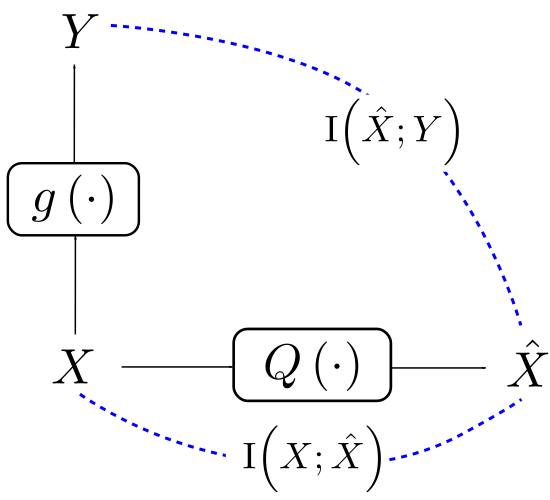
\includegraphics[width=0.4\textwidth]{information_bottleneck.pdf}
  \caption[Diagram of the Information Bottleneck.]{A diagram of variables
  relevant to the IB method. IB attempts to minimize the mutual information
between $X$ and its compressed form, $\hat{X}$, while maximizing the mutual information
between $X$ and a second variable, $Y = g(X)$. $Q$ is a function quantizing
(compressing) $X$.\label{fig:ib_diagram}}
\end{figure}

The Information Bottleneck (IB) method is a widely used technique in signal processing for
finding the optimal reduced representation $\hat{X}$ of a random variable $X$ that preserves
maximum information about a second random variable $Y$:
%
\eq{
  \Psi(p(\hat{x} \vert x))
  &=
  \min_{p(\hat{x} \vert x)}
  \
    \text{I}(X; \hat{X})
    -
    \beta
    \text{I}(\hat{X}; Y).
    \label{eq:ib_opt}
}
%
IB resembles the PRI cost functional from Section~\ref{sec:pri}, but considers the effects of
compression on the information between two datasets, as opposed to one. Similar to $\lambda$
in the PRI optimization, $\beta$ is a design parameter that trades compression for conservation
of information. As $\beta \rightarrow 0$, the optimization tends towards the trivial lossy
compression $\{\hat{X}\}=0$, whereas when $\beta \rightarrow \infty$, $\hat{X}$ approaches
its original representation $X$~\cite{principe2010information}. The two
variables in the information terms of the IB functional can equivalently be thought of as the
information loss incurred by describing $\hat{X}$ with $Y$ instead of with
$X$~\cite{geiger2011information,geiger2013signal} (Fig.~\ref{fig:ib_diagram}).

In most applications, the IB method is used to extract information relevant to $Y$ from $X$ by
iteratively refining the distribution $p(\hat{x} \vert x)$. However, given
access to a set of quantizers $\mc{Q}$ functioning on the uncompressed variable
$X$ such that $\hat{X} = Q(X)$, one may use the IB cost functional directly to select an optimal
quantization $Q^{*}$.
%
\eq{
  Q^{*}
  &=
  \argmin_{Q \in \mc{Q}}
  \
  \text{I}(X; Q(X))
  -
  \beta
  \text{I}(Q(X); Y).
  \label{eq:ib_opt2}
}
%

\section{Optimizing Map Resolution for Sensing}
\label{sec:ib_spec}

The IB method can be combined with the PRI compression strategy in
Chapter~\ref{chapter3} to determine a function, $C^{*}$, that compresses the map
as much as possible without sacrificing a significant amount of information relevant
to a sensor measurement,
$\mbf{z}$. To perform the optimization, one builds an $n$-level OG pyramid,
$\mc{C}_{n}(\mbf{m})$ (Section~\ref{sec:og_pyramid}), from the robot's map, and selects the compression that
minimizes the IB functional:
%
\eq{
  C^{*}
  &=
  \argmin_{
    C \in \mc{C}_{n}(\mbf{m})
  }
  \ \
  \text{I}_{\text{CS}}
  \left(
  \mbf{m}
  \,
  ;
  \,
  C(\mbf{m})
  \right)
  -
  \beta
  \text{I}_{\text{CS}}
  \left(
  C(\mbf{m})
  \,
  ;
  \,
  \mbf{z}
  \right).
  \label{eq:ib_arg_opt}
}
%
CSQMI is an appropriate choice for the mutual information terms in the IB
optimization, since it allows
the second term to be computed efficiently during
exploration with the formulae supplied by Charrow et
al.~\cite{charrow2015icra} (described in Section~\ref{sec:csqmi}). However, a
method for calculating the first term in~\eqref{eq:ib_arg_opt} is not yet well-defined.
It is also not yet clear what $\mbf{m}$ itself should be. Optimizing the IB functional
over the robot's entire map will cause the first term to converge onto a steady-state value
as the robot explores and learns a larger and larger map. If $\mbf{z}$ observed the entire map at
once this would not be a problem, but it is more likely that $\mbf{z}$ will only observe a small
section of the environment at a time. It is more reasonable to make $\mbf{m}$
refer to a subsection of the total map in the vicinity of the sensor measurement. This choice
allows the robot to choose a map resolution specifically tailored to locations where it is also evaluating
the reward $\text{I}_{\text{CS}}(C\left(\mbf{m}\right)\, ;\, \mbf{z})$. One sensible
choice for $\mbf{m}$ is a bounding box around the sensor measurement $\mbf{z}$.

Computing the first term in the IB functional, $\text{I}_{\text{CS}}(\mbf{m}\,
;\, C(\mbf{m}))$, requires substituting
$\mbf{m}$ and $C(\mbf{m})$ into the definition of CSQMI
in~\eqref{eq:csqmi}:
%
\eq{
  \text{I}_{\text{CS}}(\mbf{m}\, ;\, C(\mbf{m}))
  &=
  \log
  \frac
  {
    \left(\sum\limits_{\mc{M}} \sum\limits_{C(\mc{M})} p^{2}(\mbf{m}, C(\mbf{m}))\right)
    \left(\sum\limits_{\mc{M}} \sum\limits_{C(\mc{M})} p^{2}(\mbf{m}) p^{2}(C(\mbf{m}))\right)
  }
  {
    \left(
    \sum\limits_{\mc{M}} \sum\limits_{C(\mc{M})} p(\mbf{m}) p(C(\mbf{m})) p(\mbf{m}, C(\mbf{m}))
    \right)^{2}
  },
  \label{eq:csqmi_map}
}
%
where $C(\mc{M})$ is the support set of the compressed map $C(\mbf{m})$.
Due to cell independence, the sums over all possible maps reduce to products
of sums over all possible cell values, $\texttt{EMP}$ and $\texttt{OCC}$
(abbreviated $\texttt{E}$ and $\texttt{O}$):
%
\eq{
  \text{I}_{\text{CS}}(\mbf{m}\, ;\, C(\mbf{m}))
  &=
  \log
      \prod\limits_{i, j}
      \sum\limits_{o_{1}, o_{2} \in \{\texttt{E},\texttt{O}\}}
      p^{2}(\mbf{m}_{i}=o_{1}, C(\mbf{m}_{j})=o_{2})
    \\
    &+ \log
      \prod\limits_{i, j}
      \sum\limits_{o_{1}, o_{2} \in \{\texttt{E},\texttt{O}\}}
      p^{2}(\mbf{m}_{i}=o_{1}) p^{2}(C(\mbf{m}_{j})=o_{2})
    \\
    &- 2\log
      \prod\limits_{i, j}
      \sum\limits_{o_{1}, o_{2} \in \{\texttt{E},\texttt{O}\}}
      p(\mbf{m}_{i}=o_{1}) p(C(\mbf{m}_{j})=o_{2}) p(\mbf{m}_{i}=o_{1},
      C(\mbf{m}_{j})=o_{2})
  ,
  \label{eq:csqmi_map2}
}
%
with products iterating over all grid cells in the map, $i, j \in \{1,\dots,K\}$.
While $p(\mbf{m}_{i})$ and $p(C(\mbf{m}_{j}))$ are readily calculated using cell
occupancy probabilities from the uncompressed and compressed OGs, the joint distribution
$p(\mbf{m}, C(\mbf{m}))$ is not yet defined. Resurrecting the assumption that
the map can be decomposed into independent square regions
({\bf constraint 1} in Section~\ref{sec:pri_framing}) enables
the joint distribution to be represented as a product of joint distributions from independent
regions:
%
\eq{
  p(\mbf{m},C(\mbf{m}))
  &=
  \prod_{\mbf{r} \in \mbf{m}}
  p(\mbf{m}_{\mbf{r}},C(\mbf{m}_{\mbf{r}}))
  =
  \prod_{\mbf{r} \in \mbf{m}}
  p(\mbf{m}_{\mbf{r}},\tilde{\mbf{m}}_{\mbf{r}}),
  \label{eq:joint_decomp}
}
%
where $\mbf{r}$ is a vector of indices into the map $\mbf{m}$ that define a
square (or cubic) region. The second equivalence in~\eqref{eq:joint_decomp} holds
by noting that the compressed region $C(\mbf{m}_{\mbf{r}})$ has only one cell, and
that the distribution $p(\tilde{\mbf{m}}_{\mbf{r}})$ is completely determined by
knowing $p(C(\mbf{m}_{\mbf{r}}))$. $p(C(\mbf{m}_{\mbf{r}}))$ can be found by looking up the occupancy
value of the single cell in the compressed map that corresponds to the region $\mbf{r}$.

Table~\ref{tab:contingency} defines a contingency table to aid in determining
the joint distribution. The contingency table contains the random variables
$\mbf{m}^{R}$ and $\tilde{\mbf{m}}^{R}$, written here with superscripts to refer to
the cell count of the region, $R=\vert\mbf{r}\vert$. Rows in the table enumerate the
permuations that $\mbf{m}^{R}$ can take (i.e.
$\{\{\texttt{EMP},\dots,\texttt{EMP}\}$$,\dots,$
$\{\texttt{OCC},\dots,\texttt{OCC}\}\}$), while columns enumerate the
permuatations that $\tilde{\mbf{m}}^{R}$ can take (again,
$\{\{\texttt{EMP},\dots,\texttt{EMP}\}$$,\dots,$
$\{\texttt{OCC},\dots,\texttt{OCC}\}\}$). The marginal distributions
$p(\mbf{m}^{R})$ and $p(\tilde{\mbf{m}}^{R})$ are shown in the right-most column
and bottom-most row, respectively. While $p(\tilde{\mbf{m}}^{R})$ has a support
set that contains non-uniform permutations, the PRI optimization dictates that
$\tilde{\mbf{m}}^{R}$ can only take on values
$\{\texttt{EMP},\dots,\texttt{EMP}\}$ or $\{\texttt{OCC},\dots,\texttt{OCC}\}$,
since ultimately $\tilde{\mbf{m}}^{R}$ is compressed to a single cell,
$\tilde{\mbf{m}}^{1}$, taking on a value of either
$\texttt{EMP}$ or $\texttt{OCC}$
(Fig.~\ref{fig:pri_compression}).
All other permutations therefore have a marginal probability of zero.

%%%%%%%%%%%%%%%%% CONTIONGENCY TABLE %%%%%%%%%%%%%%%%%%%%%%
\begin{sidewaystable*}[Ht!]
  \caption[A contingency table for distributions relevant to occupancy grid compression.]{Contingency table for a compression from the OG region
  $\mbf{m}^{R}$ to $\tilde{\mbf{m}}^{R}$. \texttt{O} and \texttt{E} stand for \texttt{OCC} and \texttt{EMP}. \label{tab:contingency}}
    \centering
    \scalebox{0.9}
    {
    \renewcommand{\arraystretch}{3}
    \begin{tabular}{| c | c | c | c | c | c | c | c |}
        \cline{3-7}
        \multicolumn{2}{c|}{}
        & \multicolumn{1}{c}{}
        & \multicolumn{1}{c}{}
        & \multicolumn{1}{c}{$\tilde{\mbf{m}}^{R}$}
        & \multicolumn{1}{c}{}
        & \multicolumn{1}{c|}{}
        & \multicolumn{1}{c}{}
        \\ \cline{3-8}
        \multicolumn{2}{c|}{}
        & \scalebox{0.9}{\texttt{E}, \texttt{E}, $\dots$, \texttt{E}} & \scalebox{0.9}{\texttt{E}, \texttt{E}, $\dots$,
        \texttt{O}} & $\dots$ & \scalebox{0.9}{\texttt{O}, \texttt{O}, $\dots$, \texttt{E}} & \scalebox{0.9}{\texttt{O},
        \texttt{O}, $\dots$, \texttt{O}} & Total \\ \cline{1-4}\cline{6-8}
        \multirow{5}{*}{$\mbf{m}^{R}$}
        & \scalebox{0.9}{\texttt{E}, \texttt{E}, $\dots$, \texttt{E}} &
        $w_{2}\cdot(1-\tilde{\mbf{o}}^{1}) \cdot
        \prod_{i=1}^{R}(1-\mbf{o}_{i}^{R})$ & $0$ & $\dots$ & $0$ & $w_{3}\cdot
        \tilde{\mbf{o}}^{1}\cdot \prod_{i=1}^{R}(1-\mbf{o}_{i}^{R})$ &
        $\prod_{i=1}^{R}(1-\mbf{o}_{i}^{R})$\\ \cline{2-4}\cline{6-8}
        & \scalebox{0.9}{\texttt{E}, \texttt{E}, $\dots$, \texttt{O}} &
        $w_{1}\cdot(1-\tilde{\mbf{o}}^{1})\cdot \mbf{o}_{1}^{R}\cdot
        \prod_{i=2}^{R}(1-\mbf{o}_{i}^{R})$ & $0$ & $\dots$ & $0$ &
        $w_{4}\cdot\tilde{\mbf{o}}^{1}\cdot \mbf{o}_{1}\cdot
        \prod_{i=2}^{R}(1-\mbf{o}_{i}^{R})$ & $\mbf{o}_{1}\cdot
        \prod_{i=2}^{R}(1-\mbf{o}_{i}^{R})$\\ \cline{2-4}\cline{6-8}
        &
        \multicolumn{1}{c}{$\vdots$}
        &
        \multicolumn{1}{c}{$\vdots$}
        &
        \multicolumn{1}{c}{$\vdots$}
        &
        \multicolumn{1}{c}{$\ddots$}
        &
        \multicolumn{1}{c}{$\vdots$}
        &
        \multicolumn{1}{c}{$\vdots$}
        &
        \multicolumn{1}{c|}{$\vdots$} \\ \cline{2-4}\cline{6-8}
        & \scalebox{0.9}{\texttt{O}, \texttt{O}, $\dots$, \texttt{E}} & $ w_{1}
        \cdot (1-\tilde{\mbf{o}}^{1})\cdot (1-\mbf{o}_{1}^{R}) \cdot
        \prod_{i=2}^{R} \mbf{o}_{i}^{R}$ & $0$ & $\dots$ & $0$ & $w_{4}\cdot
        \tilde{\mbf{o}}^{1}\cdot (1-\mbf{o}_{1}^{R}) \cdot \prod_{i=2}^{R}
        \mbf{o}_{i}^{R}$ & $(1-\mbf{o}_{1}^{R}) \cdot \prod_{i=2}^{R} \mbf{o}_{i}^{R}$\\ \cline{2-4}\cline{6-8}
        & \scalebox{0.9}{\texttt{O}, \texttt{O}, $\dots$, \texttt{O}} &
        $w_{1}\cdot(1-\tilde{\mbf{o}}^{1})\cdot \prod_{i=1}^{R}\mbf{o}_{i}^{R}$
        & $0$ & $\dots$ & $0$ & $w_{4}\cdot\tilde{\mbf{o}}^{1}\cdot
        \prod_{i=1}^{R}\mbf{o}_{i}^{R}$ & $\prod_{i=1}^{R}\mbf{o}_{i}^{R}$ \\ \cline{1-4}\cline{6-8}
        \multicolumn{1}{c|}{}
        & Total & $1-\tilde{\mbf{o}}^{1}$ & $0$ & $\dots$ & $0$ &
        $\tilde{\mbf{o}}^{1}$ & 1 \\ \cline{2-8}
    \end{tabular}
    }
\end{sidewaystable*}



%%%%%%%%%%%%%%%%% CONTIONGENCY TABLE %%%%%%%%%%%%%%%%%%%%%%

The joint distribution $p(\mbf{m}^{R},
\tilde{\mbf{m}}^{R})$ makes up the center cells of Table~\ref{tab:contingency}.
The PRI compression strategy leaves this distribution underconstrained
by two degrees. In general, there exists an infinite set of joint distributions that satisfy
a set of marginal distributions. Two commonly used methods for constraining degrees of
freedom are choosing the joint distribution to be a product of marginals (therefore
enforcing independence between the variables), or choosing a joint distribution that
maximizes the joint entropy $\text{H}(\mbf{m}^{R}, \tilde{\mbf{m}}^{R})$~\cite{abbas2006entropy}.
In this situation, the first option will not suffice; forcing the variables to be independent of
one another will cause $\text{I}_{\text{CS}}(\mbf{m}\,;\,C(\mbf{m}))$ to be
equal to zero, eliminating all influence of the first term on the IB
optimization. The second choice is viable, but a simpler third option is
available.

The joint distribution $p(\mbf{m}^{R},\tilde{\mbf{m}}^{R})$ can instead be
chosen to be a product of the marginal distributions $p(\mbf{m}^{R})$ and $p(\tilde{\mbf{m}}^R)$, weighted
by four extra coefficients $w_{1:4}$. These coefficients are chosen to donweigh
the probability of the event that $\tilde{\mbf{m}}^{R}$ takes the value
$\{\texttt{EMP},\dots,\texttt{EMP}\}$ if any cells in $\mbf{m}^{R}$ are
occupied. This choice, similar to the heuristic $\eta$ from
Section~\ref{sec:solving_pri}, reflects the fact that occupied cells should be
preserved through compression for common operations on OGs (raycasting
and collision checking). The remaining three constants, $w_{2:4}$, balance the effects
of $w_{1}$ such that the conditional distributions $p(\mbf{m}^{R} \, \vert \,
\tilde{\mbf{m}}^{R})$ and $p(\tilde{\mbf{m}}^{R} \, \vert \, \mbf{m}^{R})$ across the rows
and columns of Table~\ref{tab:contingency} all sum to the marginal
distributions on the bottom-most row and right-most column.

With the joint distribution $p(\mbf{m}^{R}, \tilde{\mbf{m}}^{R})$ fixed, one can
compute the first term in the IB cost function~\eqref{eq:ib_arg_opt}
using~\eqref{eq:csqmi_map2}, where values for $p(\mbf{m}_{i},C(\mbf{m}_{j}))$
can be looked up from a table of computed joint probabilities.
%\end{aligned}
%\end{gather}
%
%Specficially, the
%contingency table demands that the
%coefficiencs $w_{1:4}$ are constrained to satisfy
%%
%\eq{
%  w_{2}(1-\tilde{\mbf{o}}^{1}) + w_{3}\tilde{\mbf{o}}^{1} &= 1
%  \quad \text{(first row)}
%  \\
%  w_{1}(1-\tilde{\mbf{o}}^{1}) + w_{4}\tilde{\mbf{o}}^{1} &= 1
%  \quad \text{(remaining rows)}
%  \\
%  w_{2} \prod_{i=1}^{R} (1-\mbf{o}^{R}_{i}) + w_{1} \left(1 - \prod_{i=1}^{R}
%  (1-\mbf{o}^{R}_{i})\right) &= 1
%  \quad \text{(first column)}
%  \\
%  w_{3} \prod_{i=1}^{R} (1-\mbf{o}^{R}_{i}) + w_{4} \left(1 - \prod_{i=1}^{R}
%  (1-\mbf{o}^{R}_{i})\right) &= 1
%  \quad \text{(last column)},
%}

\section{Adapting Map Compression Online}
\label{sec:adapting}

Rather than solving the IB optimization~\eqref{eq:ib_arg_opt} upon initialization
and fixing the resulting map resolution, it is necessary to adapt the map
resolution as the robot explores.
An optimal map compression in one area of the
environment is not necessarily optimal in another. For example, in a wide-open
area consisting of mostly empty cells, a map can be compressed
significantly before CSQMI between the map and a sensor measurement is altered.
Using the same amount of compression in an area cluttered with obstacles would
lead to inaccurate reward values.

The most na\"{i}ve strategy for adapting the map compression to the environment
is to reevaluate the IB optimization for each planned action. This
strategy results in the best map resolution possible for every evaluation of CSQMI
reward. However, it also completely nullifies the benefits of map compression.
The IB optimization itself requires computing CSQMI over an OG
pyramid, making this strategy more inefficient than evaluating CSQMI on the uncompressed
OG. A more useful strategy is to reperform the IB optimization whenever the robot enters a significantly
different area of the environment. Adapting to local changes in
the map requires a method for detecting such changes.

One way to detect changes in the robot's local map is to look for changes to the mean
entropy of cells in a submap where the robot is planning actions. Mean entropy is
chosen for this section, noting that other options,
such as monitoring changes to the mean or minimum distance to obstacles,
changes to the ratio of free space to occupied space in a local map, or changes
to feature-based
map descriptors can also be used. A submap can similarly be defined in many ways; for
the purposes of this section it is defined by a bounding box around the robot's
planned actions, with an added buffer for sensor range (Fig.~\ref{fig:local_map}).

\begin{figure}
  \centering
  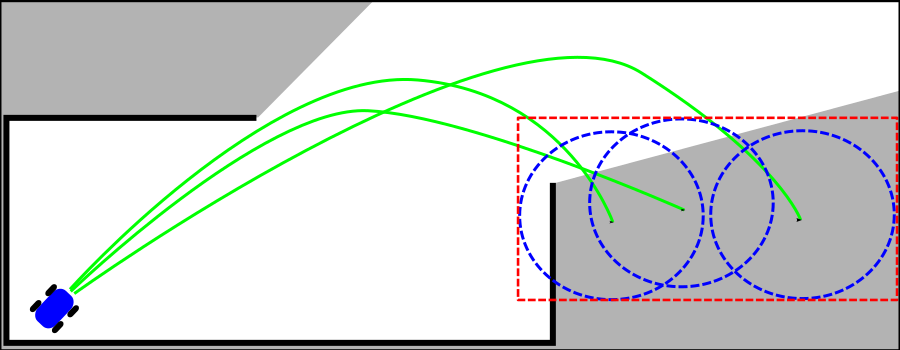
\includegraphics[width=0.8\textwidth]{local_map.pdf}
  \caption[A submap used for IB optimization.]{The mean entropy of cells in a
    submap of the robot's map is monitored to trigger IB optimizations. The submap (red) is defined by a bounding box
    around simulated sensor measurements (blue) acquired from planned actions
  (green). \label{fig:local_map}}
\end{figure}

Every time an IB optimization is performed, the mean entropy,
$\bar{\text{H}}_{\text{last}}$, of cells in the
most recent submap is cached. Afterwards, this value is continuously
monitored. A new IB optimization is triggered whenever the difference between
$\bar{\text{H}}_{\text{last}}$ and the mean entropy of cells in the current
submap surpasses a threshold, $\delta_{\text{H}} \in (0, 1)$:
%
\eq{
  \left|
  \frac{1}{\vert \bar{\mbf{m}} \vert}\sum_{i=1}^{\vert \bar{\mbf{m}} \vert}\text{H}(\bar{\mbf{m}_{i}})
  -
  \bar{\text{H}}_{\text{last}}
  \right|
  \ge \delta_{\text{H}},
  \label{eq:reoptimize}
}
%
where $\bar{\mbf{m}} \subseteq \mbf{m}$ is the robot's most recent submap.

When the criteria in~\eqref{eq:reoptimize} is met a random planned action is chosen,
and an OG pyramid is computed in the submap defined by that action. The IB optimization~\eqref{eq:ib_arg_opt}
is then performed using the computed OG pyramid and randomly selected action to
determine a new compression $C^{*}$. The new compression is
used until the criteria in~\eqref{eq:reoptimize} is met again.

Calculating the mean entropy of cells in a submap has a bounded computational
cost for actions with a fixed length, and is inexpensive in comparison to the IB
optimization itself. Large values of $\delta_{\text{H}}$ make it necessary to observe
large changes to the map before an IB optimization is retriggered.

\section{Results}

The variational parameter $\beta$ plays an influential role in the IB
optimization. Figure~\ref{fig:loss_compression} displays a multi-beam
sensor measurement simulated from the end pose of a planned action, and the IB cost
functional for varying values of $\beta$. Larger values of $\beta$ cause the
optimization to favor no map compression (therefore preserving the entire
information content of the sensor measurement). When $\beta$ is small, the
optimization is dominated by the minimum information term, and therefore favors
maximum compression.

The adaptive strategy introduced in Section~\ref{sec:adapting} was tested by
exploring a $35\times35$ m section of Carnegie Mellon University's Field Robotics
Center with a ground robot. The ground robot was equipped with a MicroStrain 3DM-GX3-35 IMU,
a Hokuyo URG-30LX $30$ m range laser scanner, and an onboard computer with an Intel Core i5
processor and 8 GB RAM (Fig.~\ref{fig:robot_platform}). The robot's hardware (motor controllers,
motors, and wheels) limit its maximum forward velocity to $1.6$ m/s.

Figure~\ref{fig:ground_experiment} shows a $72$ m
exploration path through the environment (beginning from the bottom), and the
adapted compression level and velocity estimate. Dashed lines in
Fig.~\ref{fig:ib_exploration_plots} correspond to times when the adaptation condition
in~\eqref{eq:reoptimize} is met. Colored dashed lines mark times
when~\eqref{eq:reoptimize} is met and~\eqref{eq:ib_arg_opt} computes a new
compression level $n$. The forward-arc motion primitive strategy was used for
action generation (Section~\ref{subsec:fa_motion_primitives}). Since generated primitives
expanded in the robot's forward direction, entropy was generally computed in a submap in front of
the robot. The optimal compression level remained at $4$ in most of the free regions
in the trial, and reduced to $0$, $1$, and $2$ in locations where compression results
in large reductions to CSQMI reward (e.g. the first $n=0$ region occurred as the robot
moved through a doorway). Although only a loose coupling was enforced in this experiment,
vehicle velocity was adapted in response to the robot's estimated planning frequency.
Propagating efficiency gains from map compression through to planning frequency
and velocity caused the robot to accelerate and decelerate when entering highly
compressible and incompressible areas, respectively. With no map compression,
the maximum planning frequency would have been restricted to $2$ Hz, whereas
by compressing the robot's map, the maximum
planning frequency was increased to $24$ Hz in areas with
$n=4$.

\begin{figure}
    \centering
    \begin{subfigure}[t]{0.5\textwidth}
        \centering
        \includegraphics[height=6.3cm]{plan_ahead.png}
        \caption{A simulated future sensor measurement.\label{fig:loss_compression1}}
    \end{subfigure}
    \hfill
    \begin{subfigure}[t]{0.44\textwidth}
        \centering
        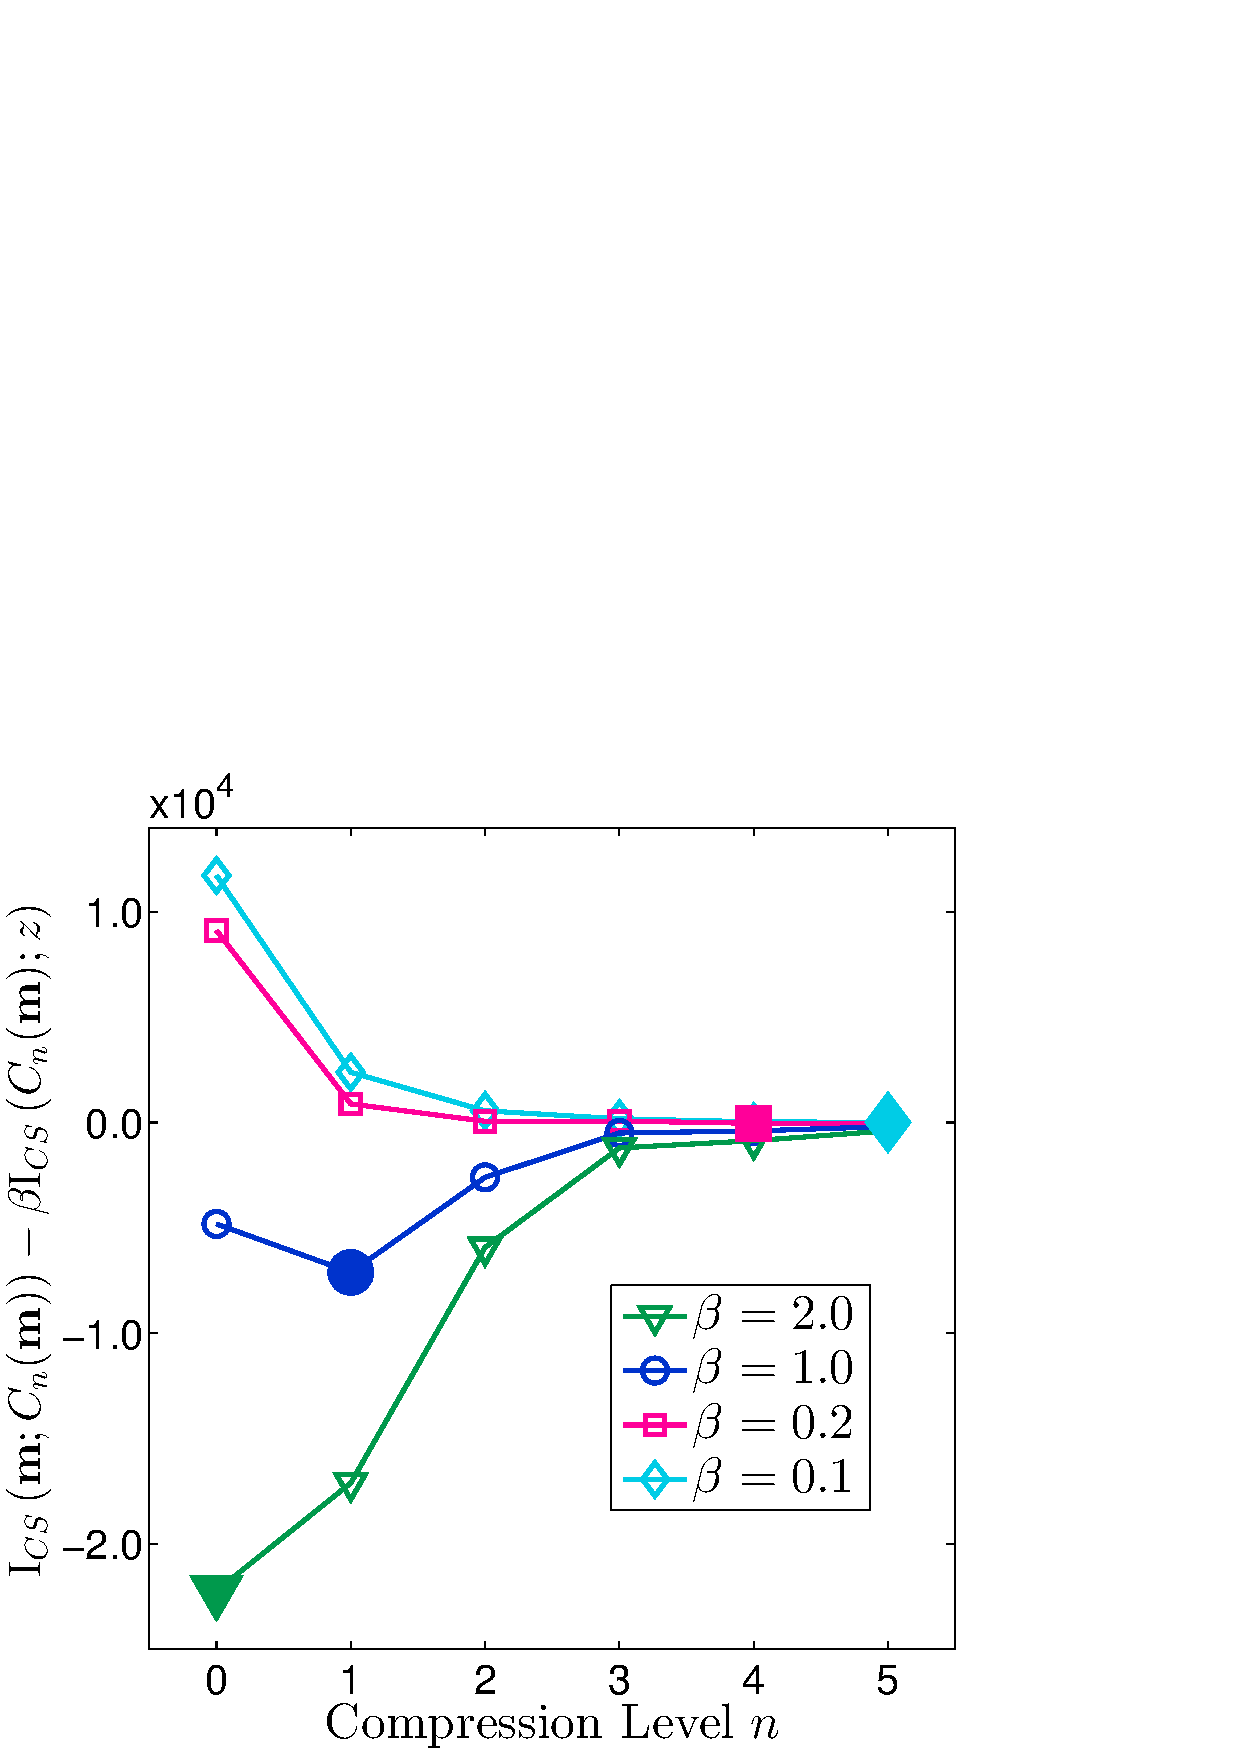
\includegraphics[height=6.5cm]{beta.pdf}
        \caption{Influence of $\beta$.\label{fig:loss_compression2}}
    \end{subfigure}
    \caption[Information Bottleneck optimization for varying values of $\beta$]{
      A sensor measurement is simulated from the endpoint of a planned action
      (Fig.~\ref{fig:loss_compression1}). The IB cost functional
      in~\eqref{eq:ib_arg_opt} is shown in Fig.~\ref{fig:loss_compression2} for
      varying values of $\beta$. The optimal compression level (filled markers)
     decreases as $\beta$ increases, favoring preservation of information about the
   measurement as opposed to compression. \label{fig:loss_compression}}
\end{figure}
%
\begin{figure}
  \centering
  \includegraphics[width=0.6\textwidth]{groundbot.jpg}
  \caption[Experimental robot platform.]{Robot platform\label{fig:robot_platform}}
\end{figure}

\begin{figure}
  \centering
    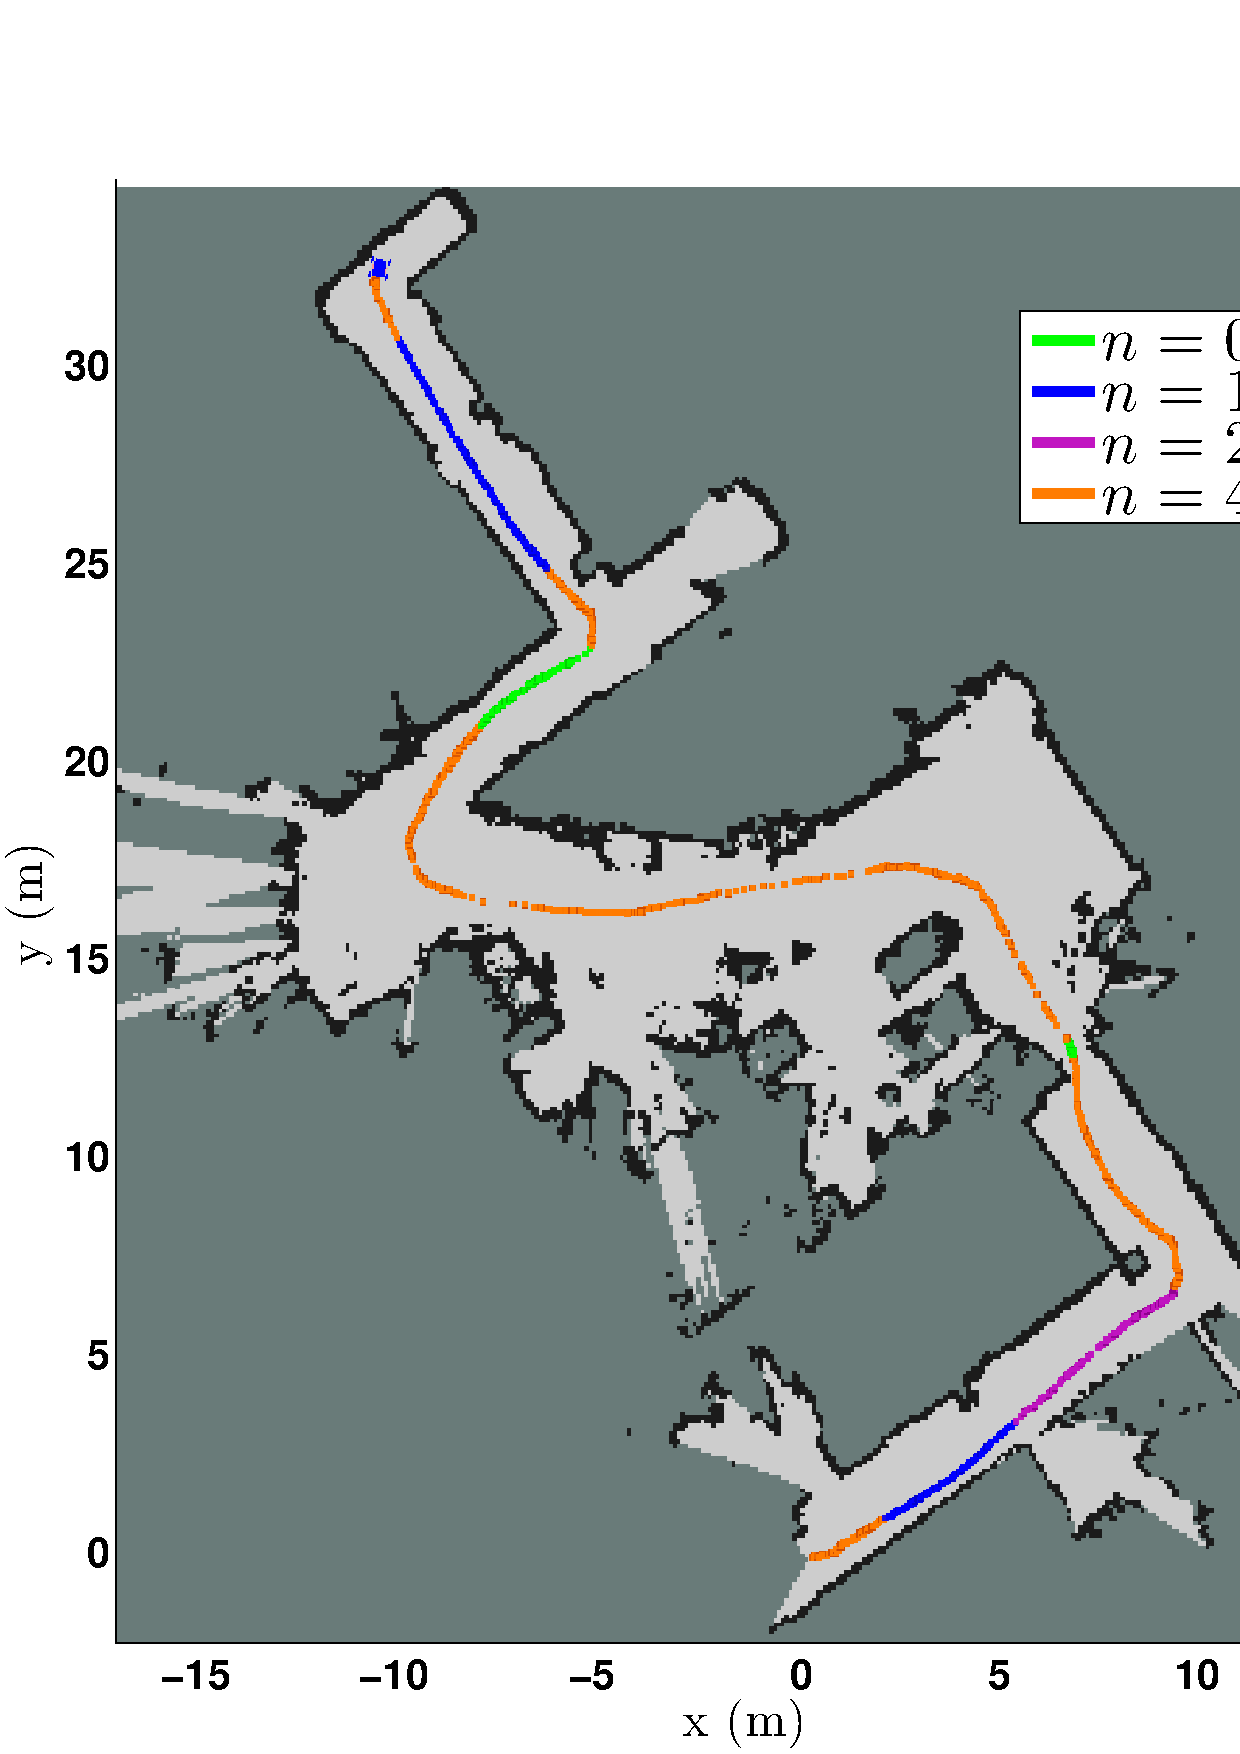
\includegraphics[width=0.9\textwidth]{ground_experiment_map2.pdf}
    \caption[Exploration path with adaptive compression.]{Ground robot
    exploration path (beginning at $(0, 0)$) with adaptive map compression.
  \label{fig:ground_experiment}}
\end{figure}

\begin{figure}
    \centering
    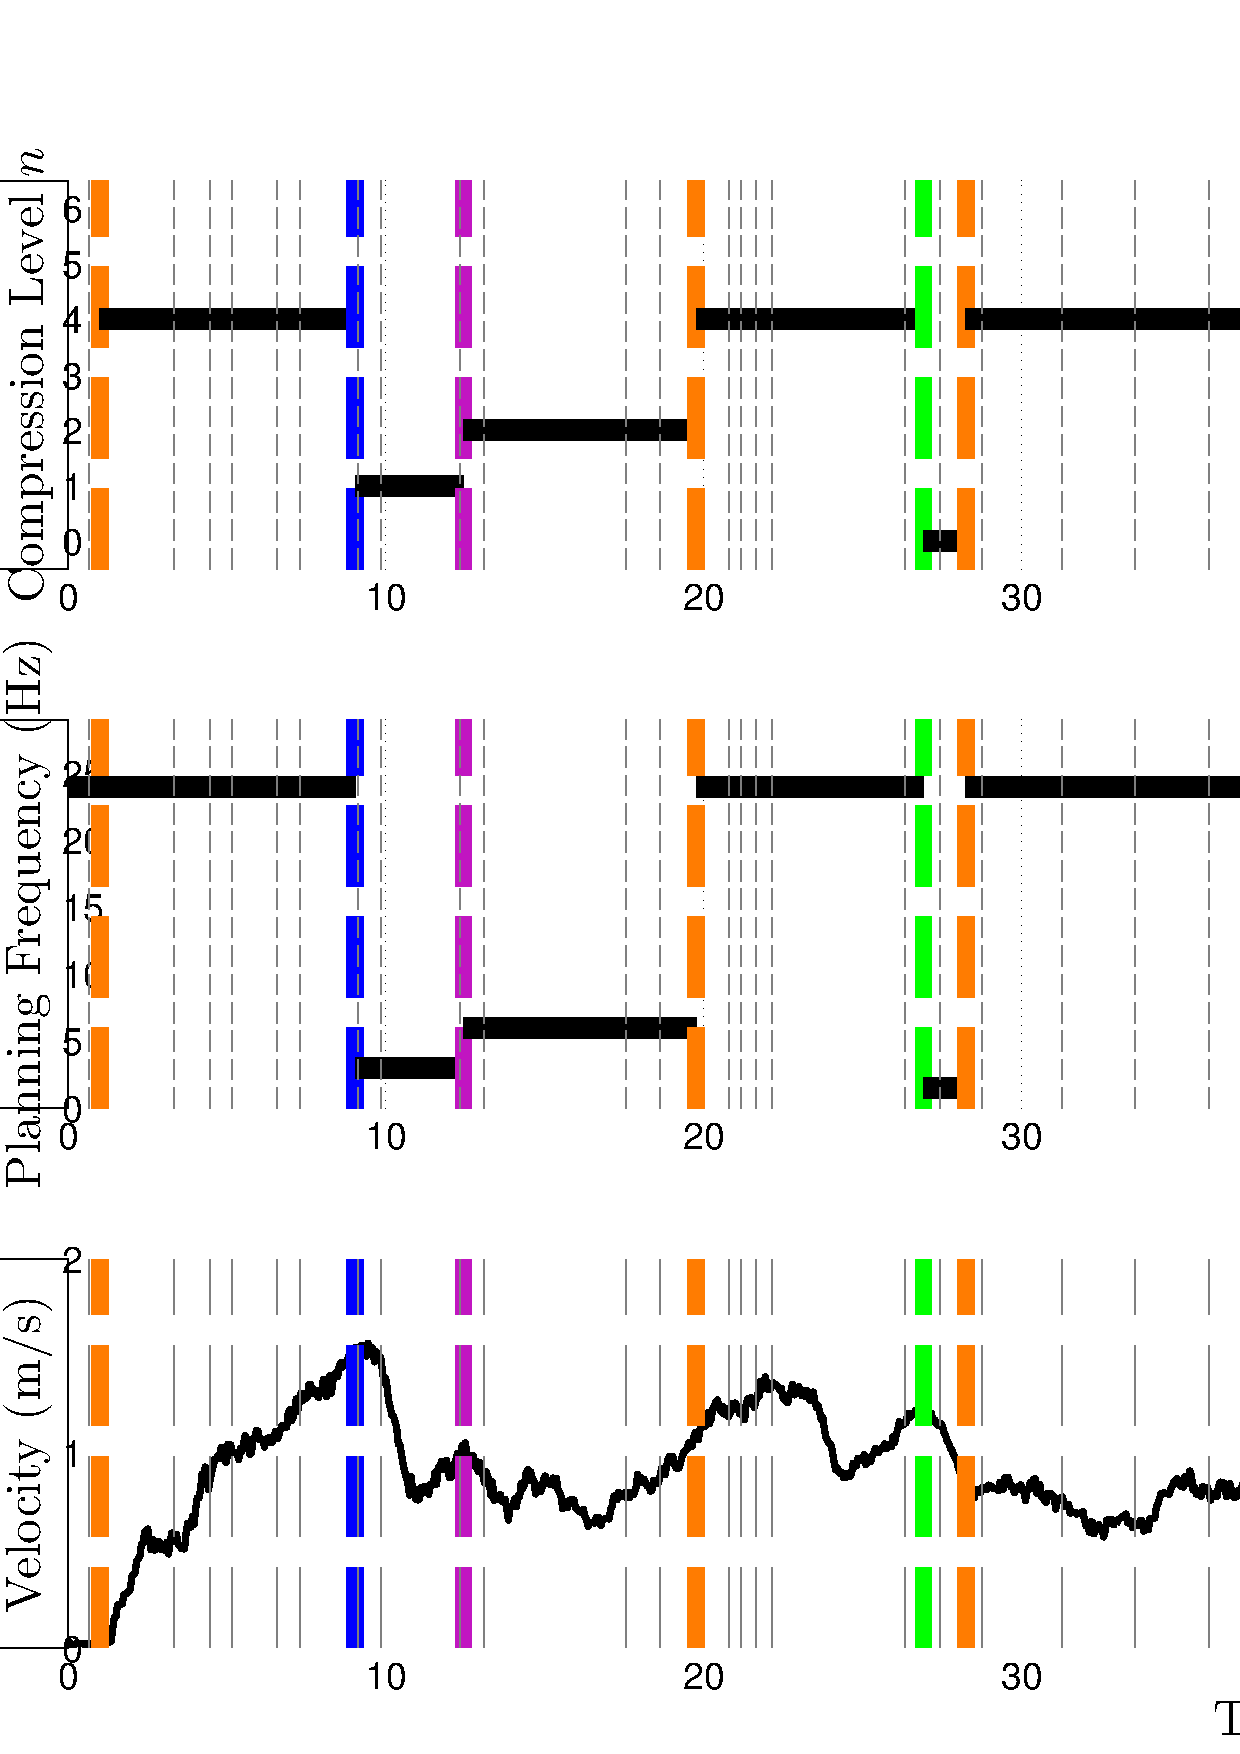
\includegraphics[width=\textwidth]{ground_plots.pdf}
    \caption{Time evolution of $n$, planning frequency, and velocity.
    \label{fig:ib_exploration_plots}}
\end{figure}

\clearpage

\section{Chapter Summary}

Chapter~\ref{chapter4} provided a strategy for choosing a map compression that simultaneously
minimizes the redundancy between the compressed and uncompressed maps, and minimizes distortion
to CSQMI between the robot's map and expected future sensor measurements. The
problem of balancing these two competing objectives was solved using the
Information Bottleneck method.

Since an exploring robot can travel through multiple distinct sections of an
environment in one deployment, the optimal map compression should be adapted
whenever the robot enters an area that is significantly different. Section~\ref{sec:adapting}
introduced an entropy-based criteria to identify when the robot's local map has changed.
Upon satisfying this criteria, an exploring robot can perform an IB optimization to
recompute an optimal map compression based on the local environment.

The IB optimization was shown to favor large map compressions for low values of
$\beta$, and no map compression for high values (Fig.~\ref{fig:loss_compression}).
A ground robot experiment was carried out to examine exploration performance with
adaptive map compression. The robot was able to adapt its map compression,
planning frequency, and velocity to changes in its local environment
(Figs.~\ref{fig:ground_experiment} and~\ref{fig:ib_exploration_plots}).
Without compressing its map, the computational cost of evaluating CSQMI limited
the robot's planning frequency to $2$ Hz. However, the adaptive map compression
strategies introduced in Chapters~\ref{chapter3} and~\ref{chapter4} allowed
for planning frequencies of up to $24$ Hz in highly compressible areas.

